\documentclass{article}
\usepackage{tikz}
\usepackage{amsmath}
\usetikzlibrary{shapes, arrows,shapes.multipart,positioning}
\tikzstyle{model} = [rectangle,rounded corners, minimum width=3cm, minimum height=1cm,text centered, draw=black,fill=red!30]
\tikzstyle{data} = [rectangle,rounded corners, minimum width=3cm, minimum height=1cm,text centered, draw=black,fill=blue!30]
\tikzstyle{result} = [rectangle,rounded corners, minimum width=3cm, minimum height=1cm,text centered, draw=black,fill=purple!30]
\tikzstyle{arrow} = [ -> ,ultra thick,>=triangle 45]

\begin{document}

\begin{figure}
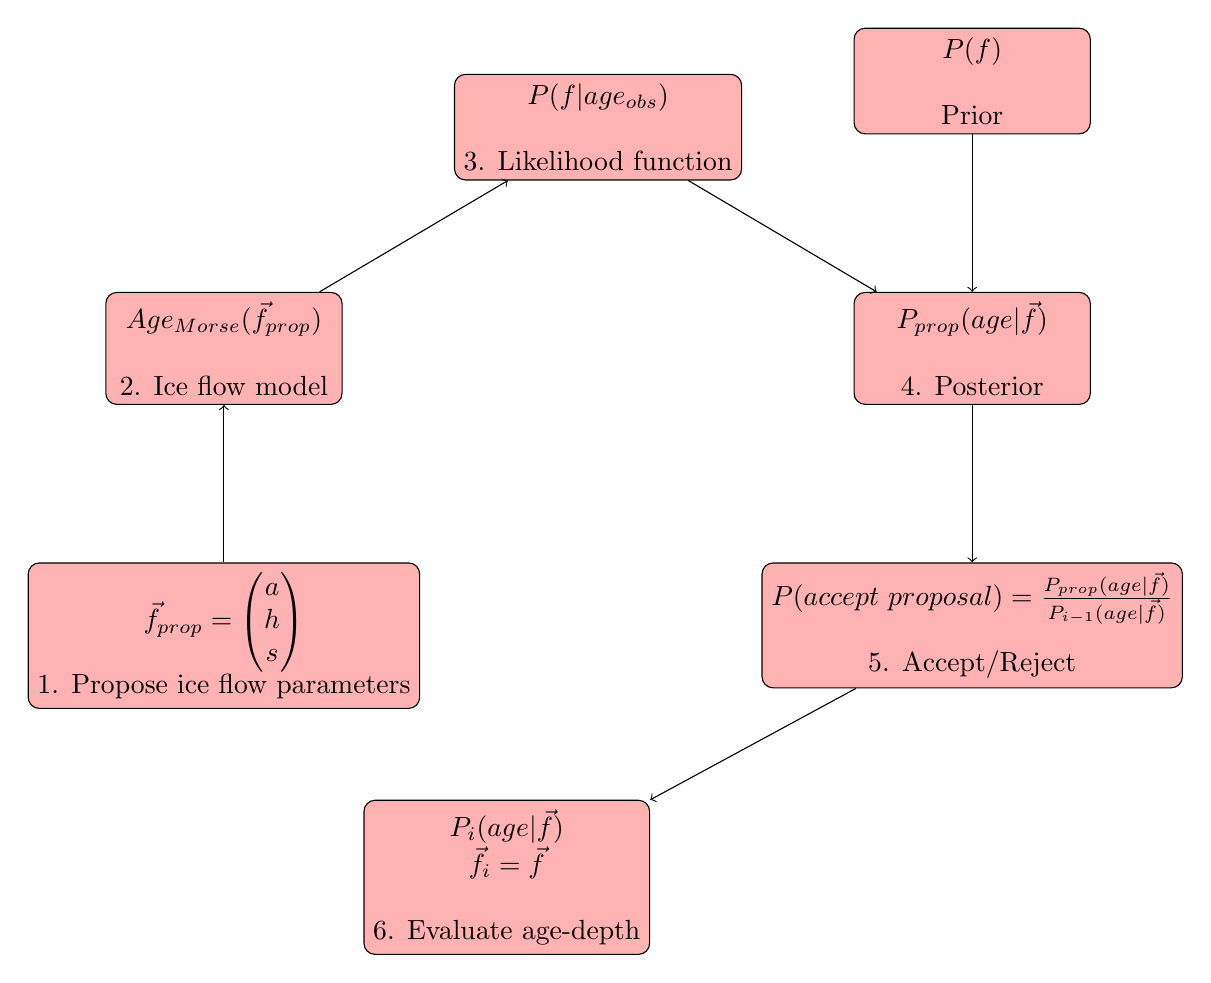
\begin{tikzpicture}[node distance=2cm,every text node part/.style={align=center}]

\node(one) [model] {$\vec{f}_{prop} = \begin{pmatrix}{a}\\h\\s\\\end{pmatrix}$
\\1. Propose ice flow parameters};

\node(two)[model,above= of one]{$Age_{Morse}(\vec{f}_{prop})$\\
\\ 2. Ice flow model};

\node(three)[model,above right = of two]{$P(f|age_{obs})$\\
\\ 3. Likelihood function};

\node(four)[model,below right = of three]{$P_{prop}(age|\vec{f})$\\ \\4. Posterior};

\node(four_a)[model,above = of four]{$P(f)$\\ \\Prior};

\node(five)[model,below = of four]{$P(accept~proposal) = \frac{P_{prop}(age|\vec{f})}{P_{i-1}(age|\vec{f})}$ \\ \\ 5. Accept/Reject};

\node(six)[model,below left = of five]{$ P_i(age|\vec{f}) $\\
$ \vec{f_i} = \vec{f}$
 \\ \\ 6. Evaluate age-depth};
%  
% \node(test)[model] {this \\ block \\ has \\ five \\ lines};
\draw[->] (four_a) edge (four);
\draw[->] (one) edge (two) (two) edge (three) (three) edge (four)(four) edge (five) (five) edge (six);


\end{tikzpicture}
\caption{}
\end{figure}

\end{document}